\chapter{Methoden}
%In the chapter Methods you describe how you proceeded to achieve the goals of your project.
%This typically contains a section about project management and a section to describe the
%theory of the used technologies. It is important to introduce and quickly explain all used
%technologies, algorithms etc., as the reader might not be familiar with them. Assume that
%the reader has a general background of IT (so words such as Software, Algorithm do not need
%to be explained), but not necessarily the same specialization (so anything specific such as git,
%deep learning etc. needs to be introduced).

% Einleitung
Das Kapitel Methoden verfügt über zwei Teile. Im Ersten zeigt es die Zusammenarbeit im Team
auf und erklärt die verwendeten Projektmethoden und Hilfsmittel.
Der zweite Teil erklärt die technische Herangehensweise sowie wichtige Konzepte und Technologien,
die für die Umsetzung von massgeblicher Bedeutung waren.

\section{Projektmanagement}

In diesem Projekt wurde keine vordefinierte Projektmethodik angewendet. Stattdessen setzten wir auf
\enquote{Best Practices} aus unseren gemeinsam durchgeführten Projekten aus der Vergangenheit, die
auf der agilen Arbeitsweise basieren, die wir aus dem Arbeitsleben gewohnt sind. Diese Konzepte und
Ideen haben wir innerhalb des Rahmens, den die Bachelor Arbeit vorgibt, genutzt und wo nötig entsprechend
ergänzt.

\subsection{Projektplanung}

Der Projektplan orientiert sich am zeitlichen und formellen Rahmen, der die BFH für die Bachelor Arbeit vorgibt und ist in vier
zum Teil überlappende Projektphasen aufgeteilt.
Die Phasen dauern alle in etwa gleich lange, doch der Fokus liegt klar auf der schriftlichen Arbeit, die am meisten
Zeit in Anspruch nimmt.
\begin{enumerate}
    \item Literaturrecherche
    \item Praxisteil
    \item Dokumentationsteil
    \item Präsentationen
\end{enumerate}

Die Abbildung \ref{gantt} bildet unseren Zeitplan in der Form eines Gantt-Diagrammes ab. In der ersten Spalte von links sind die Arbeitspakete
aufgelistet. In der zweiten die geplanten und effektiv verwendeten Zeiten. Die weiteren Spalten repräsentieren dann die zeitliche
Dimension im Projekt, dargestellt durch die nummerierten Arbeitswochen sowie dem Datum vom Montag und dem Sonntag der jeweiligen Woche.
Die fettgeschriebenen, einzeiligen Einträge in der ersten Spalte repräsentieren die Projektphasen. Deren geplante Dauer wird in dunkelblauer Farbe
angezeigt.
Jedes Arbeitspaket nimmt zwei Zeilen ein. Die erste Zeile bildet die Planung ab, die zweite die dokumentierte Realität. Die Zahlen in
der Spalte rechts des Paketnamens enthält die geplante und die effektive Zeit in Personentagen, wobei ein Personentag 8 Stunden repräsentiert.
Die farbigen Balken markieren den Zeitraum, in dem die Arbeitspakete geplant respektive durchgeführt wurden. Blau steht für die Planung und
Orange für den effektiven benötigten Zeitraum.
Die Wochen sind viergeteilt, wobei in jedem Viertel ein Personentag geleistet werden kann. Parallel abgearbeitete Arbeitspakete teilen sich diese
Zeit. Die Hälfte der Woche stellt in unserem Arbeitsplan die Spanne von Montagmorgen bis Donnerstagabend dar. Die zweite Hälfte den Zeitraum bis
zum Ende des Wochenendes.

\newpage
% \pagenumbering{gobble}
\thispagestyle{empty}
\KOMAoptions{paper=landscape,pagesize}
\recalctypearea
    \begin{figure}[H]
        \noindent
	    \begin{center}
            \makebox[\textwidth][l]{\raisebox{0pt}[15cm]{
		    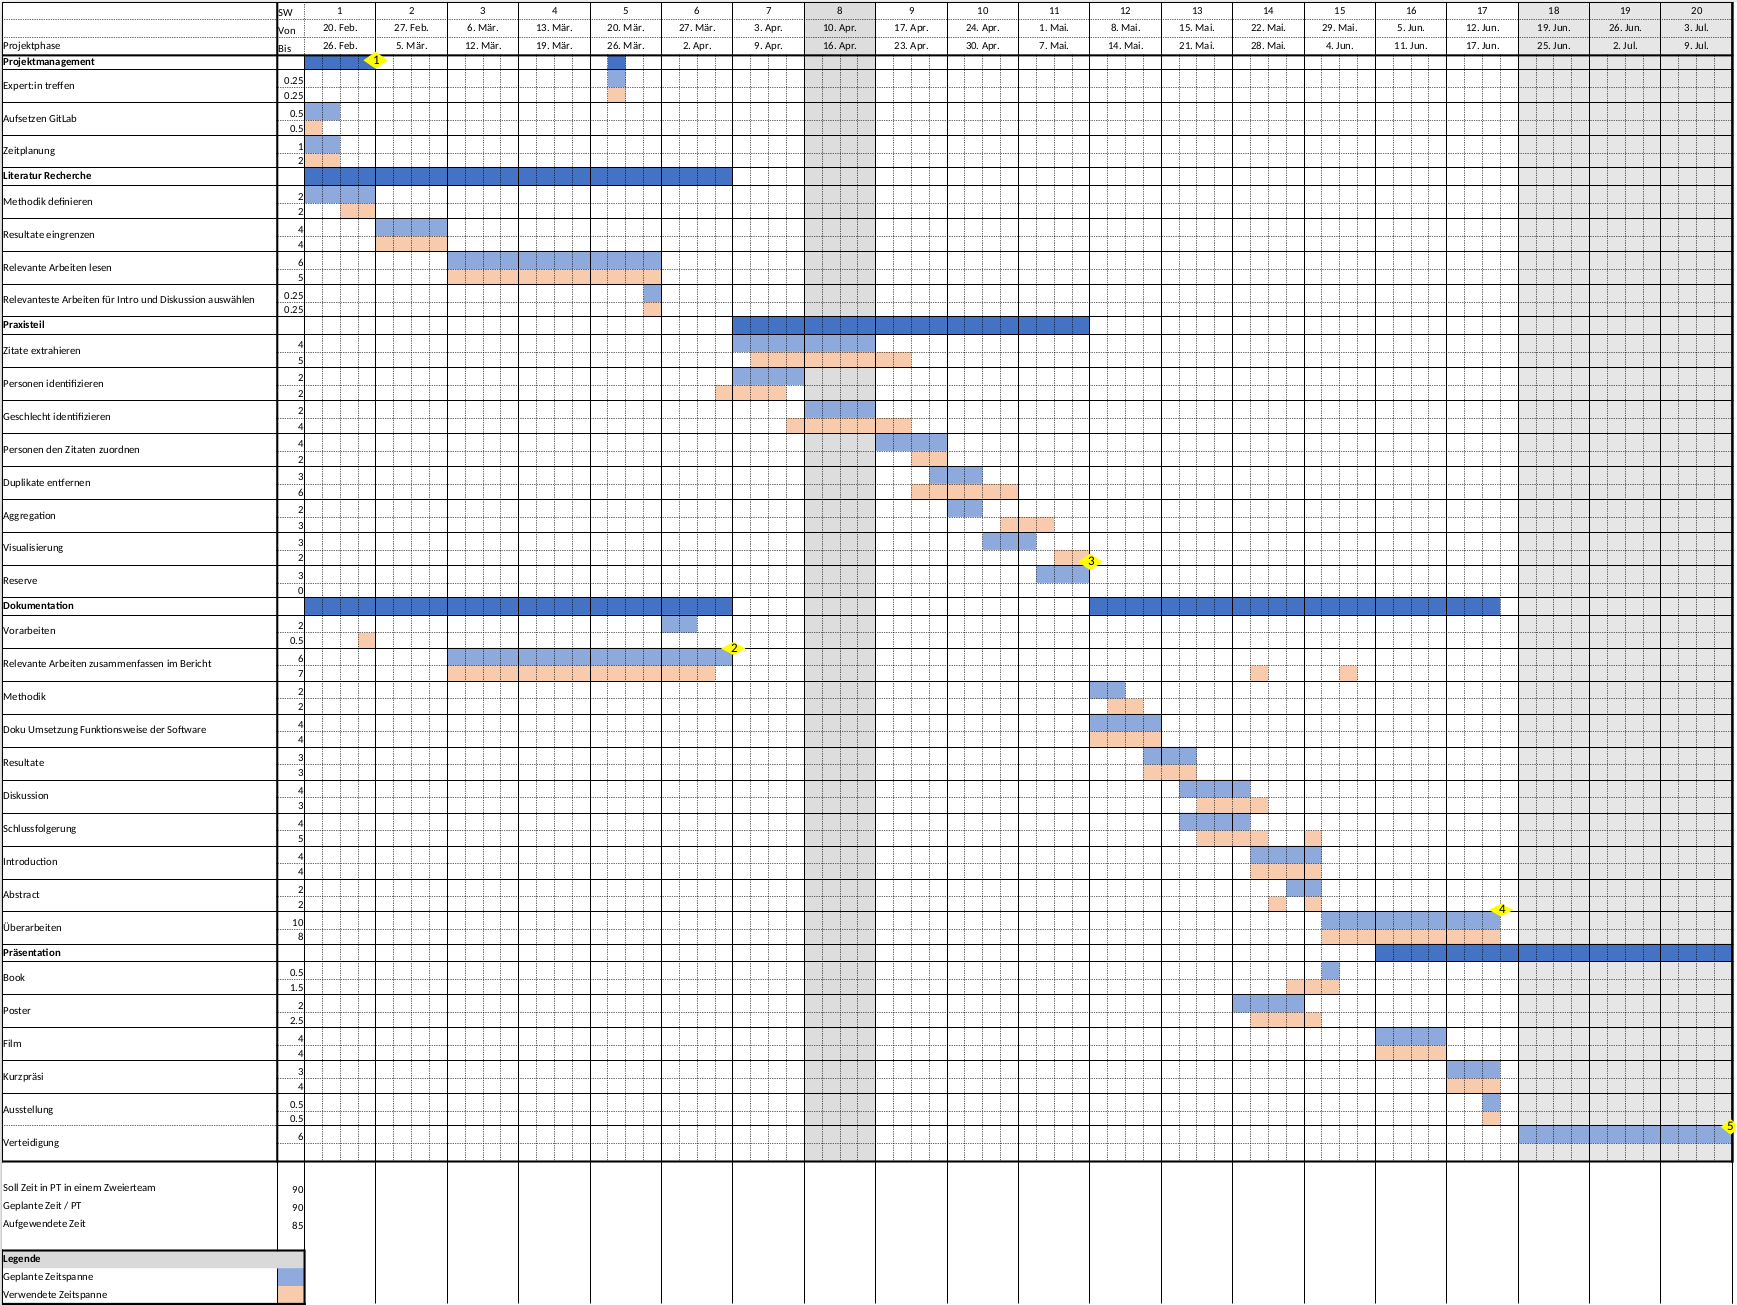
\includegraphics[width=2\linewidth,center]{images/project-planning.png}
            }}
		    \caption{Gantt Diagramm der Projektplanung}
            \label{gantt}
	    \end{center}
    \end{figure}
\newpage
% \pagenumbering{arabic}
\KOMAoptions{paper=portrait,pagesize}
\recalctypearea

\subsection{Arbeitsteilung}

Während den Besprechungen haben wir im Team die Arbeitspakete definiert und im Anschluss auf unserem
Sprint Board auf GitLab eingetragen und beschrieben. Dieses half uns, die offenen Arbeiten und Fragen
nachzuverfolgen und Doppelspurigkeiten zu Identifizieren und zu Eliminieren. Gemäss dem Projektplan haben wir
pro Projektphase ein Sprintboard erstellt, wo wir die aktuell relevanten Arbeiten stets auf einen Blick
sichtbar machen konnten. Dies half uns auch, nicht von offenen Arbeiten aus kommenden Phasen abgelenkt
zu werden. Die nachfolgende Abbildung \ref{sprint-board-screenshot} zeigt einen Screenshot vom Board der Dokumentationsphase.

\begin{figure}[H]
	\begin{center}
        \centering
		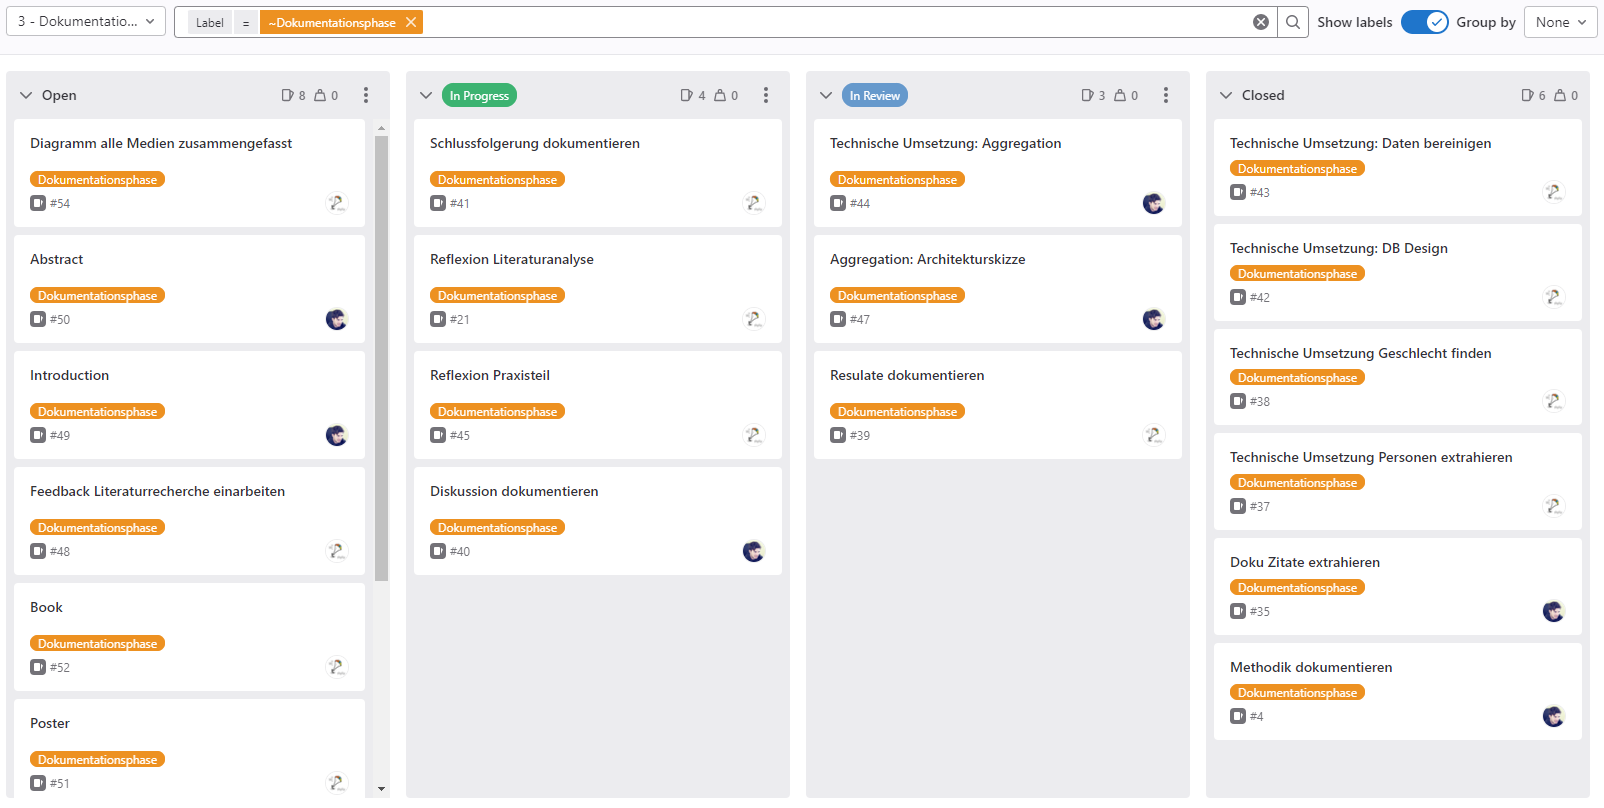
\includegraphics[width=1\linewidth]{./images/kanban_board.PNG}
		\caption{Sprint Board der Dokumentationsphase}
        \label{sprint-board-screenshot}
	\end{center}
\end{figure}

\subsection{Besprechungen}

Für die optimale Zusammenarbeit im Team waren wir stets bemüht, Entscheide gemeinsam zu fällen und
deren Ausführung im Anschluss möglichst unabhängig voneinander abschliessen zu können, um möglichst
effizient Fortschritte erzielen zu können.

Dazu trafen wir uns regelmässig am Montagabend zu einem wöchentlichen Austausch im Team, wo wir den
aktuellen Zwischenstand unserer Arbeiten, allfällige Probleme und weitere Schritte besprachen.
Zudem sahen wir uns zusätzlich stets am Freitag im Unterricht, wo wir uns informell austauschen und
neue Ideen besprechen konnten.

Zusätzlich zu den wöchentlichen Sitzungen im Kernteam trafen wir uns ungefähr jede zweite Woche mit
unserer Betreuerin, Prof. Dr. Mascha Kurpicz-Briki, um ihr den aktuellen Stand der Arbeiten und den
Fortschritt gemessen am Projektplan präsentieren zu können. In diesen Meetings konnten wir zusätzlich
inhaltliche und Formelle Fragen klären und durch Feedback von der grossen Erfahrung unserer Betreuerin
profitieren.

\section{Methoden und Konzepte zur technischen Umsetzung}

\subsection{Grundsätzliches Vorgehen}

% Einleitung + Methode P2
Das grundsätzliche Vorgehen (Methodik) wurde bereits im Vorprojekt
\cite{project2} definiert. In diesem wurden vier technische
Hauptaufgaben identifiziert, die untereinander keine oder wenige
Abhängigkeiten aufweisen. Diese resultieren in Funktionen, die auf
den gesammelten Texten oder dem Output der vorherigen Funktion operieren.
Die Abbildung \ref{dag-tasks} stellt diese Aufgaben als \gl{dag} dar.
\begin{figure}[H]
	\begin{center}
        \centering
		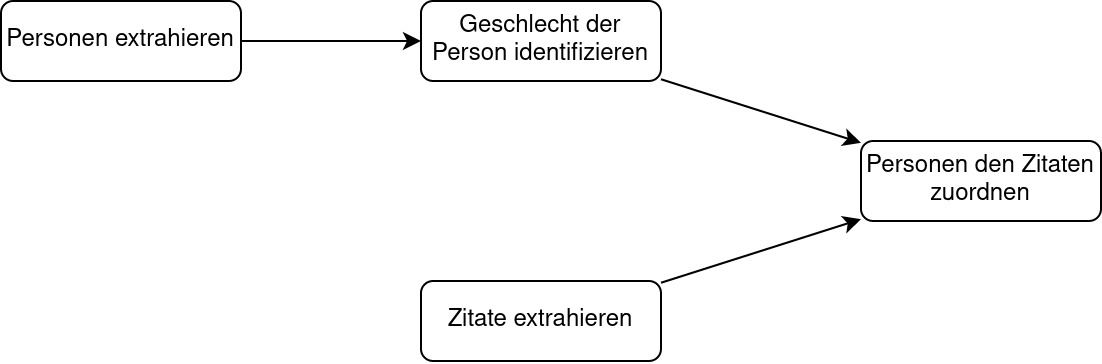
\includegraphics[width=1\linewidth]{./images/Teilaufgaben.jpg}
		\caption{\gl{dag} der Hauptaufgaben im Projekt}
		\label{dag-tasks}
	\end{center}
\end{figure}

% Zitate extrahieren
Das Extrahieren der Zitate ist von allen Teilaufgaben am unklarsten.
Teil dieser Aufgabe ist das Erkennen von eindeutigen Mustern in Zitaten
und deren Ausnutzung zur Extraktion. Der kanadische \along{ggt} (\ashort{ggt}) kann dabei
Inspiration liefern. Weil das deutsche Sprachmodell fürs \gl{dependency-parsing}
aber andere Labels verwendet als das französische und englische,
welche die Autorinnen und Autoren des kanadischen \gl{ggt} verwendet haben,
muss dieser Teil neu erfunden werden (vgl. Abschnitt \ref{citation-extraction}).

% Personen extrahieren
Die Funktion zum Extrahieren der Personen (und dazugehörigen Beschreibungen) 
wird die Software mithilfe der \gl{pos} Tagging und \gl{ner} Funktionen des \gl{spacy} Parsers umsetzen.
Die grösste Herausforderung bei dieser Aufgabe ist das \gl{cr}.
Denn für das Bestimmen des Geschlechts einer Person ist es hilfreich,
möglichst viele Aliase, Artikel und Pronomen zu kennen (vgl. Kapitel \ref{people-extraction}).

% Geschlechter bestimmen der Personen
Zum Bestimmen des Geschlechts einer Person können alle zugehörigen Informationen
verwendet werden. Am aussagekräftigsten sind Artikel und Pronomen, wobei die Zuverlässigkeit
ihrer Extraktion nicht sehr hoch ist. Ein weiteres Indiz für das Geschlecht gibt
der Vorname. Dazu wollen wir das Namensregister vom Bund zum Abfragen verwenden
\cite{bfs-vornamen-maennlich,bfs-vornamen-weiblich}. Als Backup sollen APIs aus dem
Internet dienen. Diese haben ein Rate-Limit und können nicht zu häufig abgefragt werden
(vgl. Abschnitt \ref{identify-gender}).

% Personen den Zitaten zuordnen
Als letzte Teilaufgabe gilt es, die Zitate den extrahierten Personen zuzuordnen.
Dazu wird die Position im Text und Textähnlichkeit des Namens im Zitat
und aller Eigenschaften der extrahierten Person verwendet.

% Auswertung / Aggregation
Die schlussendliche Aggregation führt für alle Artikel in der Datenbank
die bereits beschriebenen Funktionen aus und speichert das Resultat wie im 
(vgl. Kapitel \ref{db-design}).

% GG Formula
Nachdem die Software alle rund 350'000 Artikel analysiert hat, gilt es diese
auszuwerten. Das Ziel dieser Arbeit ist das Bestimmen des \gl{gendergap}s,
dem Unterschied im Raum, den Männer und Frauen in den Medien einnehmen.
Um diese klar mit einer Zahl benennen zu können, verwenden wir die abstrakte
Kennzahl \gl{gendergap} (vgl. Abschnitt \ref{ggt-formula-section}).

\subsection{Die Kennzahl \textsl{Gender Gap}}\label{ggt-formula-section}

Um den \gl{gendergap} zwischen unterschiedlichen Arbeiten vergleichen zu können,
definieren wir den \gl{gendergap} wie folgt.
Die Kennzahl repräsentiert den Unterschied im Raum, der den beiden Geschlechtern \enquote{männlich} und
\enquote{weiblich} gegeben wird, gemessen am kombinierten Anteil der Männer und Frauen.
Der \gl{gendergap} liegt deshalb stets zwischen 0 und 1,
wobei ein \gl{gendergap} von 0 eine Verteilung von 50:50 auf Männer und Frauen bedeutet
und ein \gl{gendergap} von 1 eine Verteilung des gesamten Raums auf ein Geschlecht.

Im Fall von dieser Arbeit sind mit \enquote{Raum} die Anzahl Zitate
gemeint. Die Abstraktion \enquote{Raum} ist deshalb nützlich, weil sich damit die \gl{gendergap}s
unterschiedlicher Arbeiten vergleichen lassen. So können wir beispielsweise den \gl{gendergap} des \enquote{Body Counts}
der Ringier EqualVoice Initiative \cite{ringier-equalvoice} mit unserem \gl{gendergap} anhand der
Anzahl Zitate vergleichen. Wir machen uns dies im Kapitel \ref{interpretation} zunutze, um die Ergebnisse
mit den relevantesten Arbeiten aus dem Kapitel \ref{state-of-the-art} zu vergleichen.
Keine der beigezogenen relevanten Arbeiten verfügt über eine Methodik, Formel oder Kennzahl,
mit der ein ähnlicher Vergleich möglich wäre. Die Untenstehende Formel ist ein Vorschlag,
diese Lücke zu füllen.

\begin{figure}[H]
    \begin{equation}
        Gender \, Gap = \left|\frac{RF - RM}{RF + RM}\right|
    \end{equation}
    \parbox{\linewidth}{Wobei~$RF$ der Raum ist, der Frauen gegeben wird und~$RM$ derjenige, der den Männern gegeben wird.}
    \caption{Formel zur Berechnung des \gl{gendergap}s}
    \label{ggt-formula}
\end{figure}

\subsection{Die verschiedenen Arten von Zitaten}\label{types-of-citations}

Für die Unterscheidung der Arten von Zitaten orientiert sich diese Arbeit
an der Vorbildstudie \citetitle{gender_gap_tracker} \cite{gender_gap_tracker}. Diese unterscheidet im Grundsatz
zwei Arten von Zitaten, die
\begin{enumerate}
    \item \textsl{Syntaktischen} und die
    \item \textsl{Schwimmenden Zitate}.
\end{enumerate}

Die Begründung für diese Unterscheidung ist im Kapitel \ref{ggt-method-citation} genauer
beschrieben. Was sind also \textsl{Syntaktische} und \textsl{Schwimmende} Zitate? \textsl{Syntaktische Zitate}
sind diejenigen Satzstrukturen, die alle Informationen beinhalten, die zu einem Zitat gehören:
\begin{enumerate}
    \item Ein Zitat in der direkten oder indirekten Rede
    \item Ein Subjekt, das zitiert wurde
    \item Ein Zitat-einleitendes Verb
\end{enumerate}
Ein Beispiel dafür ist \enquote{Der Bundesrat Berset versicherte, dass genügend Masken vorhanden seien.} oder \enquote{Der Bundesrat Berset versicherte: \enquote{Es sind genügend Masken vorhanden.}}.
In diesem Beispiel ist das Zitat \enquote{dass genügend Masken vorhanden seien} beziehungsweise \enquote{Es sind genügend Masken vorhanden}. Das Subjekt ist in beiden Fällen
\enquote{Der Bundesrat Berset}. Auch das einleitende Verb ist in diesen Fällen gleich, nämlich \enquote{versicherte}.

\textsl{Schwimmende Zitate} finden sich besonders in Texten, in denen eine Person mehrfach zitiert und das Subjekt nicht jedes Mal wiederholt wird.
Um beim vorherigen Beispiel zu bleiben, können wir uns eine Weiterführung des Textes so vorstellen: \enquote{Der Bundesrat Berset versicherte, dass genügend Masken vorhanden seien.
\enquote{Es sind genug für alle da.}}. Das Zitat \enquote{\enquote{Es sind genug für alle da.}} \textsl{schwimmt} im Text ohne selbst von einem Verb eingeleitet oder im selben Satz
von einem Subjekt begleitet zu werden. Für uns Menschen ist damit implizit klar, dass das Zitat zu der zuvor zitierten Person gehört.
Für einen Algorithmus sind solche impliziten Muster schwieriger zu erkennen und zu verbinden, weshalb solche \textsl{Schwimmenden Zitate} anders behandelt werden
müssen.


\subsection{Technologien}

Die folgenden Abschnitte erklären die Grundsätze der verwendeten Technologien.

\subsubsection{Python}
Die Applikation nutzt Python der Version 3.10, eine schwach typisierte 
Skriptsprache, die aufgrund ihrer Flexibilität eine schnelle Entwicklung
auch für grössere Anwendungen ermöglicht und dank ihres reichen Ökosystems
viele Verwendungsmöglichkeiten bietet. Diese Flexibilität bringt jedoch
auch gewisse Herausforderungen mit sich, wie z.B. die Abwesenheit von
Typen und Klammern, welche die
Zusammenarbeit im Team erschweren können. Aus diesem Grund wurde in
diesem Projekt für den produktiven Code der PEP8 Standard eingehalten und mit MyPy
eine Typisierung durchgesetzt. Diese beiden Eigenschaften stellen wir
durch Linting in der GitLab Pipeline (vgl. Abschnitt \ref{gitlab}) sicher.

\subsubsection{Git}
Git ist ein verteiltes Versionskontrollsystem, das bei der Verwaltung
von Quellcode und dessen Änderungen hilft. Entwickler:innen können mit
Git Änderungen an Code vornehmen, ihre Arbeit mit anderen teilen und
zusammenarbeiten. Git bietet auch Funktionen wie Branching und Merging,
um komplexe Entwicklungsaufgaben zu unterstützen. 

\subsubsection{GitLab}\label{gitlab}
GitLab ist eine Webanwendung, die auf Git aufbaut und ein umfangreiches
Set von Tools für die Zusammenarbeit an Softwareprojekten bereitstellt.
GitLab bietet Funktionen wie Projektmanagement, Issue-Tracking,
Continuous Integration / Continuous Deployment (CI/CD) und vieles mehr,
um die Entwicklung von Software zu erleichtern.

Die BFH hostet eine eigene Instanz von GitLab, auf der wir unser Repository
\footnote{https://gitlab.ti.bfh.ch/aesca4/bachelor-thesis-2023-gender-gap-tracker-schweizer-medien}
veröffentlicht haben.

In unserem Projekt haben wir GitLab Pipelines eingesetzt, um die
Codequalität mittels Linting sicherzustellen und das LaTeX Dokument
zu builden, sodass stets eine gültige Version verfügbar ist.
Die Abbildung \ref{fig:pipeline} zeigt die drei Jobs, die wir dafür verwenden.

\begin{figure}[H]
	\begin{center}
		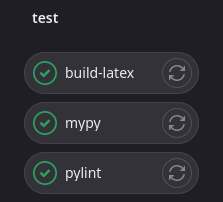
\includegraphics[width=0.5\columnwidth]{./images/gitlab-pipeline.PNG}
		\caption{GitLab Pipeline Web Crawler}
		\label{fig:pipeline}
	\end{center}
\end{figure}

\subsubsection{MongoDB}\label{mongoDB}

MongoDB ist eine dokumentenorientierte NoSQL-Datenbank, die auf flexible
Datenmodellierung und Skalierbarkeit ausgelegt ist. Im Gegensatz zu
relationalen Datenbanken verwendet MongoDB keine Tabellen, sondern
speichert Daten in Dokumenten, die in \gl{collection}s organisiert sind.
Dies ermöglicht eine einfache Handhabung von unstrukturierten Daten
und eine schnelle Abfrage von Informationen. Diese Eigenschaften
ermöglichten uns eine schnelle und flexible Entwicklung des Programmcodes.

MongoDB bietet auch ein umfangreiches Set von Funktionen wie Aggregation,
Indexierung und Volltextsuche.

Ausführlichere Informationen zu MongoDB sind auf der offiziellen Webseite
\footnote{https://www.mongodb.com/} zu finden. Zum Einbinden des Treibers
und der Verwendung mittels Python haben wir öffentlich zugängliche Tutorials
der offiziellen Seite von MongoDB\footnote{https://pymongo.readthedocs.io/en/stable/index.html}
und der Seite GeeksForGeeks \footnote{https://www.geeksforgeeks.org/python-mongodb-tutorial/} verwendet.

\subsubsection{Natural Language Processing (NLP)}

Natural Language Processing (NLP) beschäftigt sich mit der Verarbeitung
von natürlicher Sprache durch Computer und ermöglicht es, diese in eine
für Maschinen verständliche Form zu bringen. Dabei kommen
Algorithmen und Techniken zum Einsatz, die es ermöglichen, Texte zu
verstehen, zu analysieren und zu generieren. Dazu werden häufig Libraries
wie \gl{spacy} (vgl. Abschnitt \ref{spacy}) oder NLTK \footnote{https://www.nltk.org/} verwendet.

\subsubsection{Named Entity Recognition (NER)}

\gl{ner} ist eine \gl{nlp} Technologie und ermöglicht
das automatische Identifizieren von Entitäten mit Namen wie Personen,
Orten, Organisationen und Produkten in Texten. Die in diesem Projekt
geschriebene Software verwendet \gl{ner} von \gl{spacy}

\subsubsection{Part Of Speech (POS) Tagging}

\gl{pos} Tagging ist eine \gl{nlp} Funktionalität, die dazu dient, die Wortarten
(Nomen, Verb, Adjektiv...) aller Wörter in einem Satz zu bestimmen.
Im Allgemeinen werden für \gl{pos} \gl{ml} gestützte Programme verwendet,
um die Zuordnung der Wörter zu den jeweiligen Kategorien zu bestimmen.

\subsubsection{Coreference Resolution}

\gl{cr} ist eine Technik der Sprachanalyse, die darauf abzielt, Pronomen, Artikel und Synonyme im Text
auf ihre Referenz im selben Text zu beziehen. Sie identifiziert das Substantiv, auf das
sich ein Wort bezieht, um eine eindeutige Bedeutung des Satzes
zu ermöglichen. Coreference Resolution ist ein wichtiger Schritt bei der 
automatisierten Textanalyse und ermöglicht es, die Bedeutung von Texten besser zu 
verstehen. In dem Fall dieses Projekts ermöglicht die Zuordnung der Pronomen zu
den Personen eine effizientere Bestimmung des Geschlechts der Person. Da diese
zum Teil Hinweise zum Geschlecht einer Person enthalten (er, sie, sein, ihr...).

\subsubsection{Dependency Parsing}

Dependency Parsing ist eine Technik des \gl{nlp}s, die Beziehungen
zwischen Wörtern in einem Satz untersucht und hierarchisch darstellt.
Dabei wird jeder Satz in eine Baumstruktur umgewandelt, in dem jedes
Wort einen Knoten darstellt und die Beziehungen zwischen den Wörtern durch
Kanten dargestellt werden. Die Beziehungen sind abhängig von der Bedeutung
des Satzes und geben an, welches Wort mit welchem anderen Wort zusammenhängt.

\subsubsection{Spacy}\label{spacy}

\gl{spacy} ist eine Open-Source-Bibliothek für \gl{nlp}, die in Python geschrieben wurde.
Sie bietet Entwickler:innen eine Vielzahl von Funktionen zur Verarbeitung von
Texten, einschliesslich Tokenisierung, \gl{pos}-Tagging, \gl{ner} und
\gl{dependency-parsing}. Spacy wurde für hohe Leistung und Geschwindigkeit entwickelt
und ist auf die Verarbeitung grosser Textmengen ausgelegt. Die Library verfügt über Modelle,
die in mehreren Sprachen verfügbar sind und es ermöglichen, Texte in verschiedenen
Sprachen zu verarbeiten.

In unserem Projekt haben wir das Spacy Modell \enquote{de\_core\_news\_lg}
\footnote{https://spacy.io/models/de/\#de\_core\_news\_lg} verwendet, um die
Funktionen \gl{ner}, \gl{pos}-Tagging und \gl{dependency-parsing} auf deutschsprachige
Texte anzuwenden.